\documentclass{VUMIFPSkursinis}
\usepackage{algorithmicx}
\usepackage{algorithm}
\usepackage{algpseudocode}
\usepackage{amsfonts}
\usepackage{amsmath}
\usepackage{bm}
\usepackage{caption}
\usepackage{color}
\usepackage{float}
\usepackage{graphicx}
\usepackage{listings}
\usepackage{subfig}
\usepackage{wrapfig}
\usepackage{multirow}
\usepackage{longtable}
\usepackage{array,makecell}
\usepackage{enumitem}

% Titulinio aprašas
\university{Vilniaus universitetas}
\faculty{Matematikos ir informatikos fakultetas}
\department{Programų sistemų katedra}
\papertype{Programų sistemų inžinerija}
\title{Keleivių kontrolės paieškos programėlė}
\titleineng{AVOID A TICKET}
\status{2 kurso 5 grupės studentai}
\author{Elena Reivytytė}
\secondauthor{Matas Šilinskas}
\thirdauthor{Kasparas Taminskas}
\fourthauthor{Aidas Vaikšnoras}
\fifthauthor{Tadas Žaliauskas}
\supervisor{dr. Vytautas Valaitis}
\date{Vilnius – \the\year}

% Nustatymai
% \setmainfont{Palemonas}   % Pakeisti teksto šriftą į Palemonas (turi būti įdiegtas sistemoje)
\bibliography{bibliografija}

\begin{document}
\maketitle

\sectionnonum{Anotacija}
Dokumente pateikiamas ICONIX programų kūrimo proceso pirmojo etapo aprašas, kuriame aprašoma statinė programos struktūra, išreikšta supaprastinta klasių diagrama, kurioje yra tik agregacijos ir generalizacijos ryšiai, ir panaudojamumo atvejų tekstai, nurodantys, kaip sistema turi funkcionuoti. Šiame etape pateikiamas projektuojamos sistemos modelis tebėra verslo abstrakcijų lygmenyje, todėl išreikštų sistemos dalių (atributų, metodų, kitų sąveikos elementų) čia nenurodoma.

\tableofcontents

\sectionnonum{Įvadas}
\noindent
\textbf{Programų sistemos pavadinimas}\\
Programėlės pavadinimas AvoidATicket išvertus iš anglų kalbos reiškia „Nepirk bilieto be reikalo“\\
\textbf{Dalykinė sritis}\\
Programėle, kurioje viešojo transporto keleiviai gali dalintis informacija apie vykdomas viešojo transporto bilietų patikras.\\
\textbf{Probleminė sritis}\\
Programėlė yra skirta padėti klientams sutrumpinti kelionių laiką parodant, kuriose vietose keleivių kontrolė tikrina autobusus.\\
\textbf{Vartotojas}\\
Klientas - bet kokio amžiaus žmogus, kuris turi išmanųjį telefoną ir naudojasi miestinių autobusų teikiamomis paslaugomis.\\
\textbf{Darbo pagrindas}\\
Tikslas ištirti rinką galimam programėlės vystymui. Taip pat programėlės projektavimas teoriniame lygmeny siekiant supaprastint programavimo darbus.\\
\textbf{Darbo pagrindas}\\
\begin{tabular}{lr}
   Elena Reivytytė & 20\% \\
   Aidas Vaikšnoras & 20\% \\
   Kasparas Taminskas & 20\% \\
   Tadas Žaliauskas & 20\% \\
   Matas Šilinskas & 20\% \\
\end{tabular}

\section{Poreikiai}
\begin{enumerate}[itemsep=-2mm]
	\item Vartotojas gali prisijungti, atsijungti ir registruotis prie programėlės.
	\item Vartotojas turi galimybę prisijungti naudojantis “Facebook” paskyra.
	\item Vartotojas gali keisti registracijos metu įvestus duomenis: vardą, pavardę, el. paštą, slaptažodį, prisijungimo vardą.
	\item Vartotojas gali pridėti žymeklį, nurodantį vietą, kurioje yra kontrolė netoliese nuo jo esančiu atstumu (1500 metrų).
	\item Vartotojas balsuodamas gali patvirtinti arba paneigti, kad žymeklio vietoje stovi keleivių kontrolė.
	\item Vartotojas gali sekti dominančius transporto maršrutus ir realiu laiku stebėti, kuriose maršruto stotelėse stovi kontrolė. 
	\item Vartotojas gali peržiūrėti kitų vartotojų padėtus žymeklius. 
	\item Vartotojas gali palikti komentarą apie žymeklį. 
	\item Vartotojas gali perskaityti D.U.K. programėlėje.
	\item Vartotojas gali užduoti klausimą.
	\item Administratorius gali keisti kiekvieno vartojo vardą, pavardę, el. paštą, slaptažodį, prisijungimo vardą.
	\item Administratorius gali pridėti naują vartotoją ir administratorių.
	\item Programėle turi būti anglų kalba. 
	\item Padėti žymekliai rodomi tik tam tikrą laiko tarpą.
	\item Administratorius gali ištrinti bet kurį vartotojo pažymėtą žymeklį.
	\item Išjungus programėlę, vartotojas liekas prisijungęs.
\end{enumerate} 

\section{Reikalavimai}
\subsection{Funkciniai reikalavimai }
Šiame skyriuje pateikiami sistemos funkciniai reikalavimai, t.y. pagrindinės sistemos atliekamos funkcijos, konkretūs jų aprašymai.

\newcounter{frcount}
\newcommand\rownumberfr{\stepcounter{frcount}\arabic{frcount}}

\begin{longtable}{ | >{\centering}m{2cm} | m{10cm} | >{\centering}m{2.5cm} | } \caption{Funkciniai reikalavimai.} \endhead \hline
\multicolumn{3}{ |l| }{\textbf{Funkciniai reikalavimai:}} \tabularnewline \hline
\textbf{Numeris} & \centering{\textbf{Reikalavimas}} & \textbf{Svarba} \tabularnewline \hline

FR\rownumberfr & Įsijungęs programėlę, vartotojas gali:
						\begin{enumerate}[itemsep=-2mm]
							\item registruotis
							\item prisijungti
							\item neteisingai įvedęs duomenis, vartotojas gali pasitaisyti
						\end{enumerate}
				\textit{Žr. skyrius poreikiai, 1 punktas} & Būtina\tabularnewline \hline

FR\rownumberfr & Prisijungęs vartotojas gali atsijungti.\newline \textit{Žr. skyrius poreikiai, 1 punktas} & Būtina\tabularnewline \hline
FR\rownumberfr & Vartotojas gali prisijungti naudodamas “Facebook” paskyrą.\newline \textit{Žr. skyrius poreikiai, 2 punktas} & Būtina\tabularnewline \hline
FR\rownumberfr & Savo paskyroje vartotojas gali keisti:
						\begin{enumerate}[itemsep=-2mm]
							\item slaptažodį
							\item vardą
							\item pavardę
							\item prisijungimo vardą
							\item el. paštą
						\end{enumerate}
				\textit{Žr. skyrius poreikiai, 3 punktas} & Būtina\tabularnewline \hline
FR\rownumberfr & Vartotojas gali pridėti žymeklį, nurodantį vietą, kurioje yra kontrolė netoliese nuo jo esančiu atstumu.
				 \newline \textit{Žr. skyrius poreikiai, 4 punktas} & Būtina\tabularnewline \hline
FR\rownumberfr & Vartotojas gali balsuoti ar žymeklis yra klaidingas ar ne.\newline \textit{Žr. skyrius poreikiai, 5 punktas} & Būtina\tabularnewline \hline
FR\rownumberfr & Vartotojas Vartotojas gali sekti dominančius transporto maršrutus ir realiu laiku stebėti, kuriose maršruto stotelėse stovi kontrolė.\newline \textit{Žr. skyrius poreikiai, 6 punktas} & Būtina\tabularnewline \hline
FR\rownumberfr & Vartotojas gali peržiūrėti kitų vartototojų padėtus žymeklius.\newline \textit{Žr. skyrius poreikiai, 7 punktas} & Būtina\tabularnewline \hline
FR\rownumberfr & Vartotojas gali palikti komentarą prie žymeklio.\newline \textit{Žr. skyrius poreikiai, 8 punktas} & Būtina\tabularnewline \hline
FR\rownumberfr & Vartotojas gali perskaityti D.U.K. pačioje programėlėje.\newline \textit{Žr. skyrius poreikiai, 9 punktas} & Būtina\tabularnewline \hline
FR\rownumberfr & Vartotojas gali užduoti klausimą pačioje programėlėje.\newline \textit{Žr. skyrius poreikiai, 10 punktas} & Būtina\tabularnewline \hline

FR\rownumberfr & Administratorius gali pakeisti bet kurio vartotojo:
						\begin{enumerate}[itemsep=-2mm]
							\item slaptažodį
							\item vardą
							\item pavardę
							\item prisijungimo vardą
							\item el. paštą
						\end{enumerate}
				\textit{Žr. skyrius poreikiai, 11 punktas} & Būtina\tabularnewline \hline
FR\rownumberfr & Administratorius gali pridėti naują vartotoją arba administratorių.\newline \textit{Žr. skyrius poreikiai, 12 punktas} & Būtina\tabularnewline \hline
FR\rownumberfr & Padėti žymekliai rodomi 1h 30min skaičiuojant nuo padėjimo laiko, o vėliau yra automatiškai ištrinami.\newline \textit{Žr. skyrius poreikiai, 14 punktas} & Būtina\tabularnewline \hline
FR\rownumberfr & Administratorius gali ištrinti visus žymeklius.\newline \textit{Žr. skyrius poreikiai, 15 punktas} & Būtina\tabularnewline \hline
FR\rownumberfr & Išjungus programėlę, vartotojas liekas prisijungęs.\newline \textit{Žr. skyrius poreikiai, 16 punktas} & Būtina\tabularnewline \hline
\end{longtable}

\subsection{Nefunkciniai reikalavimai}
Šiame skyriuje pateikiami nefunkciniai reikalavimai sistemoms, t.y. reikalavimai, tiesiogiai nesusiję su sistemos atliekamomis funkcijomis.

\newcounter{nfrcount}
\newcommand\rownumber{\stepcounter{nfrcount}\arabic{nfrcount}}

\subsubsection{OS reikalavimai}
\begin{longtable}{ | >{\centering}m{2cm} | m{10cm} | >{\centering}m{2.5cm} | } \caption{Nefunkciniai OS reikalavimai} \endhead \hline
\multicolumn{3}{ |l| }{\textbf{OS reikalavimai:}} \tabularnewline \hline
\textbf{Numeris} & \centering{\textbf{Reikalavimas}} & \textbf{Svarba} \tabularnewline \hline
NFR\rownumber & Programėlė turi būti palaikoma Android (nuo 4.0 versijos) įrenginiuose & Būtina\tabularnewline \hline
NFR\rownumber & Programėlė palaikoma iOS (nuo 8.0 versijos) įrenginiuose. & Pageidautinas\tabularnewline \hline
NFR\rownumber & Aplikacija turi būti pasiekiama ir be išmanaus telefono - per naršyklę & Būtina\tabularnewline \hline
NFR\rownumber & Išmanusis renginys turi turėti GPS modulį. & Būtina\tabularnewline \hline
NFR\rownumber & Išmanusis įrenginys turi turėti prieigą prie interneto & Būtina\tabularnewline \hline
\end{longtable}

\subsubsection{Saveikos su  kitomis programomis reikalavimai}
\begin{longtable}{ | >{\centering}m{2cm} | m{10cm} | >{\centering}m{2.5cm} | } \caption{Nefunkciniai saveikos su  kitomis programomis reikalavimai} \endhead \hline
\multicolumn{3}{ |l| }{\textbf{Saveikos su  kitomis programomis reikalavimai:}} \tabularnewline \hline
\textbf{Numeris} & \centering{\textbf{Reikalavimas}} & \textbf{Svarba} \tabularnewline \hline
NFR\rownumber & Facebook ir Google api vartotojo autorizacijai & Būtina\tabularnewline \hline
NFR\rownumber & Aplikacija reikalauja GPS prieigos teisių. & Būtina\tabularnewline \hline
NFR\rownumber & Aplikacija reikalauja priegos prie mobiliojo interneto, jei neprisijungta prie Wi-Fi. & Būtina\tabularnewline \hline
NFR\rownumber & Google api žaidimo vietos nustatymui. & Būtina\tabularnewline \hline
\end{longtable}

\subsubsection{Programavimo aplinkos reikalavimai}
\begin{longtable}{ | >{\centering}m{2cm} | m{10cm} | >{\centering}m{2.5cm} | } \caption{Nefunkciniai programavimo aplinkos reikalavimai} \endhead \hline
\multicolumn{3}{ |l| }{\textbf{Programavimo aplinkos reikalavimai:}} \tabularnewline \hline
\textbf{Numeris} & \centering{\textbf{Reikalavimas}} & \textbf{Svarba} \tabularnewline \hline
NFR\rownumber & Programėlė kuriama C\# programavimo kalba. & Būtina\tabularnewline \hline
NFR\rownumber & Kodo versijavimui ir dalinimuisi naudojama Github repozitorija. & Būtina\tabularnewline \hline
\end{longtable}

\subsubsection{Tikslumo reikalavimai}
\begin{longtable}{ | >{\centering}m{2cm} | m{10cm} | >{\centering}m{2.5cm} | } \caption{Nefunkciniai tikslumo reikalavimai duomenų saugojimui} \endhead \hline
\multicolumn{3}{ |l| }{\textbf{Tikslumo reikalavimai duomenų saugojimui:}} \tabularnewline \hline
\textbf{Numeris} & \centering{\textbf{Reikalavimas}} & \textbf{Svarba} \tabularnewline \hline
NFR\rownumber & Vartotojo informacijai skiriama:
						\begin{enumerate}[itemsep=-2mm]
							\item vardui, pavardei ir prisijungimo vardui - 15 simbolių
							\item slaptažodžiui - 20 simbolių
							\item el. paštui - 60 simbolių
						\end{enumerate}
			  & Būtina\tabularnewline \hline
NFR\rownumber & Vartotojo prisijungimo vardas ir slaptažodis turi susidaryti bent iš 5 simbolių. & Būtina\tabularnewline \hline
NFR\rownumber & Kiekvieno vartotojo slaptažodis privalo turėti bent vieną didžiąją raidę ir bent vieną skaičių. & Būtina\tabularnewline \hline
NFR\rownumber & Vartotojo prisijungimo vardas turi būti unikalus. & Būtina\tabularnewline \hline
NFR\rownumber & Programėlėje esantis tekstas rašomas anglų kalba. \newline \textit{Žr. skyrius poreikiai, 13 punktas} & Būtina\tabularnewline \hline
\end{longtable}

\subsubsection{Aptarnavimo ir priežiūros reikalavimai}
\begin{longtable}{ | >{\centering}m{2cm} | m{10cm} | >{\centering}m{2.5cm} | } \caption{Nefunkciniai aptarnavimo ir priežiūros reikalavimai} \endhead \hline
\multicolumn{3}{ |l| }{\textbf{Aptarnavimo ir priežiūros reikalavimai:}} \tabularnewline \hline
\textbf{Numeris} & \centering{\textbf{Reikalavimas}} & \textbf{Svarba} \tabularnewline \hline
NFR\rownumber & Į vartotojo užduodamus klausimus darbo metu turi būti atsakyta ne vėliau nei per valandą, o ne darbo metu ne vėliau nei per 12 valandų. & Pageidautina\tabularnewline \hline
NFR\rownumber & Praplėtus sistemos funkcionalumą, būtina testuoti atnaujinimus, kad būtų užtikrinta programėlės sklandi veikla, prieš leidžiant jais naudotis registruotiems vartotojams, svečiams ir administratoriui. & Būtina\tabularnewline \hline
NFR\rownumber & Testai turi padengti 80\% kodo. & Būtina\tabularnewline \hline
NFR\rownumber & Programėlę galima atsinaujinti per Google Play. & Būtina\tabularnewline \hline
\end{longtable}

\subsubsection{Dalykinės srities metaforų reikalavimai}
\begin{longtable}{ | >{\centering}m{2cm} | m{10cm} | >{\centering}m{2.5cm} | } \caption{Nefunkciniai dalykinės srities metaforų reikalavimai} \endhead \hline
\multicolumn{3}{ |l| }{\textbf{Dalykinės srities metaforų reikalavimai:}} \tabularnewline \hline
\textbf{Numeris} & \centering{\textbf{Reikalavimas}} & \textbf{Svarba} \tabularnewline \hline
NFR\rownumber & Žymeklių duomenys (koordinates ir padėjimo laikas) saugomi duomenų bazėje. & Būtina\tabularnewline \hline
NFR\rownumber & Vartotojas gali padėti ne daugiau 10 žymeklių per dieną. & Būtina\tabularnewline \hline
\end{longtable}

\section{Statinė programų sistemos struktūra}	
\subsection{Esybių diagrama}
	\begin{figure}[H]
				\centering
				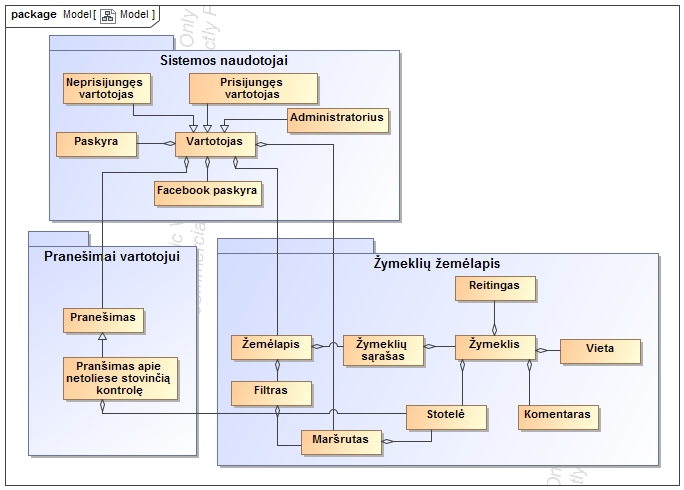
\includegraphics[scale=0.6]{img/esybiu_diagrama}
				\caption{Esybių diagrama}
				\label{img:Esybių diagrama}
			\end{figure}
\subsection{Reikalavimų - esybių atsekamumo matrica}
	\begin{figure}[H]
				\centering
				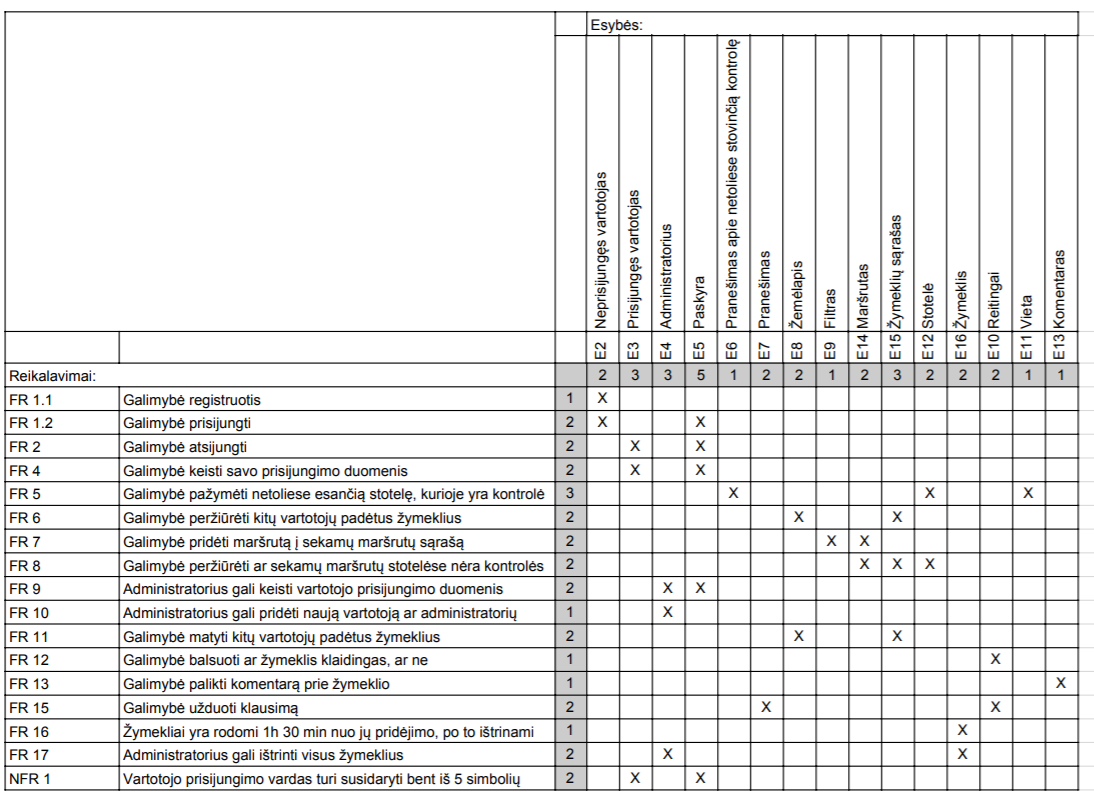
\includegraphics[scale=0.4]{img/esybiu_matrica}
				\caption{Reikalavimų atsekamumo matrica}
				\label{img:matrix}
			\end{figure}

\subsection{Žodynas}
				\renewcommand{\labelitemi}{$\bullet$}
				\begin{itemize}[itemsep=-2mm]
					\item \textit{Vartotojas} - klientas, prisiregistravęs prie aplikacijos.
					\item \textit{Neprisijungęs vartotojas} - vartotojas, kuris nėra atlikęs prisijungimo procedūros programėlėje ir neturi galiojančios prisijungimo sesijos.
					\item \textit{Prisijungęs vartotojas} - vartotojas, sėkmingai atlikęs prisijungimo procedūrą programėlėje ir turintis galiojančią prisijungimo sesiją.
					\item \textit{Administratorius} - vartotojas, atsakingas už sklandų programėlės veikimą, turintis padidintas teises paprastų vartotojų atžvilgiu.
					\item \textit{Paskyra} - registracijos metu kliento nurodyti duomenys (vardas, pavardė, elektroninio pašto adresas, prisijungimo vardas, slaptažodis), padedantys identifikuoti klientą.
					\item \textit{Facebook paskyra} - registracijos metu kliento autentifikacijai naudota paskyra.
					\item \textit{Pranešimas} - sistemos informacinė žinutė vartotojui naudojant Android pranešimus (angl. push notifications).
					\item \textit{Žemėlapis} - virtualus žemėlapis, kuriame matomi visi vartotojų pažymėti aktyvūs žymekliai, atitinkantys vartotojo nustatytą paieškos filtrą.
					\item \textit{Filtras} - savybė, pagal kurią filtruojama, kurių stotelių žymeklius vartotojui rodyti žemėlapyje.
					\item \textit{Reitingas} - žymeklio patikimumo rodiklis, žymintis pagal vartotojų balsus nustatomą tikimybę, kad žymeklio vietoje stovi keleivių kontrolė. 
					\item \textit{Vieta} - GPS prieigos pagalba tiksliai nustatytos objekto buvimo koordinatės.
					\item \textit{Stotelė} - vieta, pro kurią reguliariai kursuoja viešasis transportas.
					\item \textit{Komentaras} - vartotojo nurodyta papildoma informacija apie žymeklio vietoje stovinčią keleivių kontrolę.
					\item \textit{Maršrutas} - tam tikro autobuso kelionės metu aplankomų stotelių sąrašas.
					\item \textit{Keleivių kontrolė} - kontrolieriai, tikrinantys, ar keleiviai turi galiojančius ir tinkamos nuolaidų grupės bilietus
					\item \textit{Programėlė} - aplikacija, kurioje vartotojas gali pamatyti ar pažymėti žemėlapių vietas, kuriose yra keleivių kontrolė.
					\item \textit{Facebook} - socialinis tinklas “Facebook”.
				\end{itemize}
\subsection{Užduotys}
	\begin{figure}[H]
				\centering
				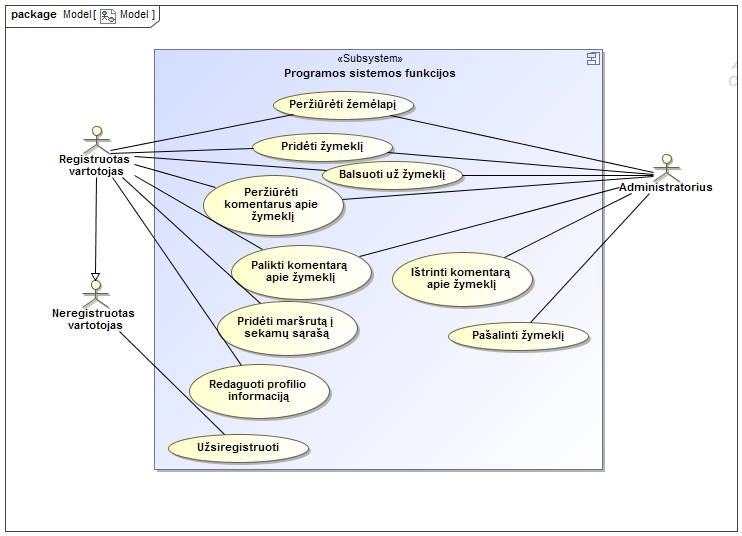
\includegraphics[scale=0.5]{img/uzduotys}
				\caption{Užduotys}
				\label{img:uzduotys}
			\end{figure}

\subsection{Užduočių aprašai}
\subsubsection{Registracija}
	Šiame skyriuje aprašomas vartotojo registracijos procesas, kuris yra schematizuotas robastiškumo diagramoje (žr. \ref{img:Registracijos robustiškumo diagrama} pav.). 
	Procesą iliustruoja registracijos lango maketas (žr. \ref{img:registracija} pav.).

	\textbf{Pagrindinis scenarijus:}\\
	Vartotojas įsijungia programėlę ir patenka į prisijungimo langą. Joje spaudžia mygtuką “Register” ir patenka į registracijos langą. 
	Registracijos lange vartotojas įveda prisijungimo vardą, savo vardą, pavardę, el. paštą, slaptažodį, slaptažodį pakartoja bei paspaudžia 
	“Create my account”. Anketa sėkmingai sukuriama, vartojo įvesti duomenys išsaugomi duomenų bazėje ir vartotojas perkeliamas į prisijungimo langą.

	\textbf{Alternatyvūs scenarijai:}
	\begin{enumerate}[itemsep=-2mm]
		\item Jei vartotojo įvestame prisijungimo varde nėra 5 simbolių, programa pateikia informacinį pranešimą, kad prisijungimo vardas netinkamas, nes jame turi būti bent 5 simboliai.
		\item Jei vartotojo įvestas prisijungimo vardas duomenų bazėje jau egzistuoja, tada vartotojui programa pateikia informacinį pranešimą, kad prisijungimo vardas netinkamas, nes jau yra vartotojas su tokiu prisijungimo vardu.
		\item Jei vartotojo įvestas prisijungimo vardas yra per ilgas, tada vartotojui programa pateikia informacinį pranešimą, kad prisijungimo vardas netinkamas, nes prisijungimo vardas negali būti ilgesnis nei 15 simbolių eilutė.
		\item Jei įvestame varde ar pavardėje yra skaičių, programa pranešą, kad vardas arba pavardė yra nevalidūs.
		\item Jei vartotojo įvestas el. paštas neatitinka el. pašto formato, programa informuoja vartotoją, kad įvestas el. paštas netinkamas.
		\item Jei įvestame slaptažodyje nėra skaičiaus ar didžiosios raidės, arba jis yra trumpesnis nei 5 simboliai, tada vartotojui programa pateikia informacinį pranešimą, kad slaptažodis netinkamas, jame privalo būti didžioji raidė ir skaičius ir kad jį turi sudaryti bent 5 simboliai. Jei  vartotojo įvestas slaptažodis yra per ilgas, tada vartotojui programa pateikia informacinį pranešimą, kad slaptažodis netinkamas, nes slaptažodis negali būti ilgesnis nei 20 simbolių eilutė.
		\item Jei slaptažodžio bei slaptažodžio pakartojimo laukai nesutampa, tada vartotojui programa pateikia informacinį pranešimą, kad įvesti slaptažodžiai nesutampa.
		\item Jei dėl trikdžių duomenų bazėje vartotojui prisiregistruoti nepavyksta, tada vartotojui programa pateikia informacinį pranešimą, kad sistemoje įvyko klaida ir siūloma pabandyti prisiregistruoti vėliau.
	\end{enumerate} 
		\begin{figure}[H]
				\centering
				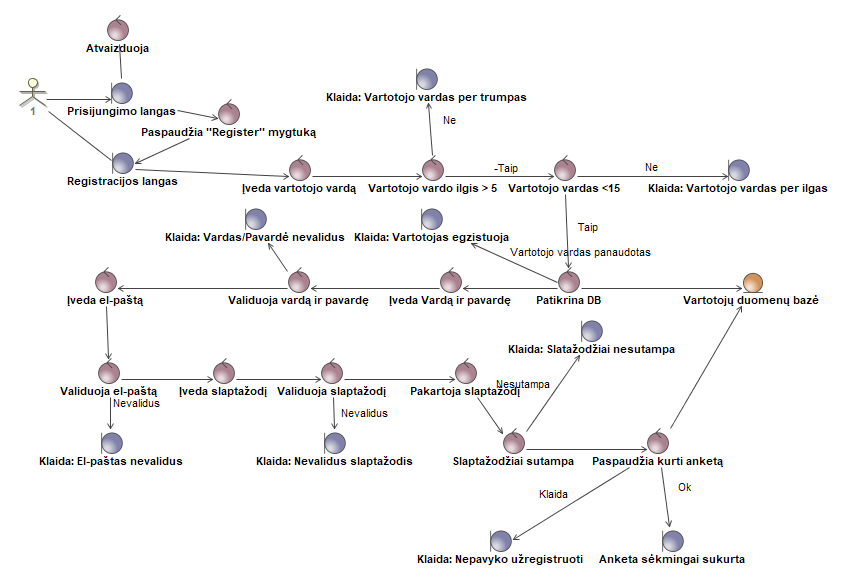
\includegraphics[scale=0.55]{img/Robustness_Registracija}
				\caption{Registracijos robustiškumo diagrama}
				\label{img:Registracijos robustiškumo diagrama}
			\end{figure}
	\begin{figure}[H]
				\centering
				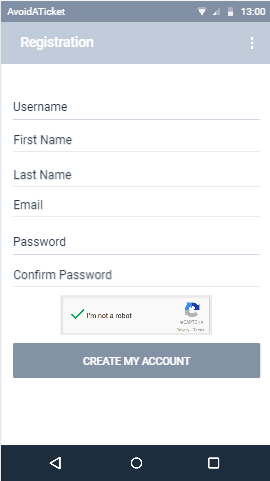
\includegraphics[scale=0.55]{img/mockup_registration}
				\caption{Registracijos lango maketas}
				\label{img:registracija}
			\end{figure}

\subsubsection{Prisijungimas}
	Šiame skyriuje aprašomas vartotojo prisijungimo prie aplikacijos procesas, kuris yra schematizuotas robastiškumo diagramoje (žr. \ref{img:Prisijungimo robustiškumo diagrama} pav.). 
	Procesą iliustruoja prisijungimo lango maketas (žr. \ref{img:prisijungimas} pav.).

	\textbf{Pagrindinis scenarijus:}\\
	Vartotojas įsijungia programėlę ir patenka į prisijungimo langą. Prisijungimo lange įveda savo prisijungimo vardą ir slaptažodį, 
	spaudžia mygtuką “Login”, prisijungia ir yra perkeliamas į pagrindinį langą.
	
	\textbf{Alternatyvūs scenarijai:}
	\begin{enumerate}[itemsep=-2mm]
		\item Jei vartotojas praeitą sesiją neatsijungė, tada programėlė automatiškai prijungia vartotoją prie programėlės ir iškart vartotoją perkelia į pagrindinį langą.
		\item Jei vartotojas su tokiu prisijungimo vardu duomenų bazėje nebuvo rastas, tada vartotojui programa pateikia informacinį pranešimą, kad vartotojas su tokiu prisijungimo vardu programėlėje neegzistuoja.
		\item Jei vartotojo įvestas slaptažodis šiam prisijungimo vardui nesutampa su slaptažodžiu, esančiu sistemoje, tada vartotojui programa pateikia informacinį pranešimą, kad įvestas slaptažodis yra neteisingas.
		\item Jei vartotojas prisijungimo lange spaudžia “Continue with Facebook” ir vartotojo “Facebook” programėlės anketa sėkmingai panaudojama prisijungimui prie “AvoidATicket” programėlės, tada vartotojas yra prijungiamas ir perkeliamas į pagrindinį langą.
		\item Jei vartotojas prisijungimo lange spaudžia “Continue with Facebook” ir vartotojo “Facebook” programėlės anketos nepavyksta panaudoti prisijungimui prie “AvoidATicket” programėlės, tada vartotojui programa pateikia informacinį pranešimą, kad “Facebook” aplikacijos prisijungimo duomenų panaudoti nepavyko.
		\item Jei dėl trikdžių duomenų bazėje vartotojui prisijungti nepavyksta, tada vartotojui programa pateikia informacinį pranešimą, kad sistemoje įvyko klaida ir siūloma pabandyti prisijungti vėliau.
	\end{enumerate} 
	\begin{figure}[H]
				\centering
				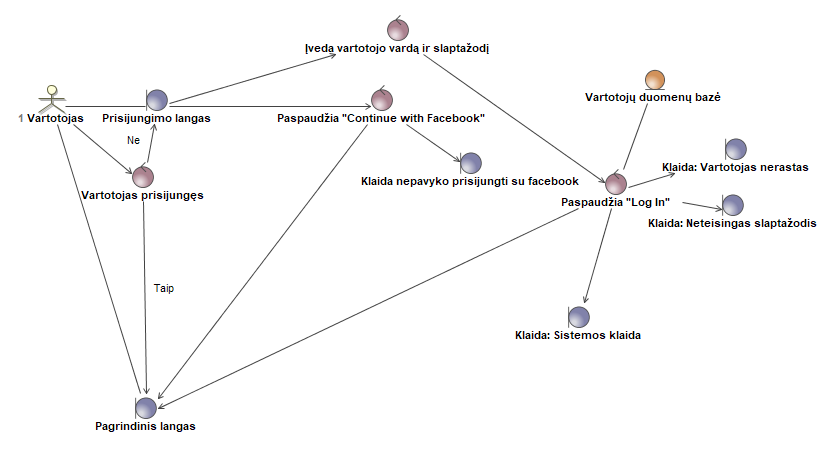
\includegraphics[scale=0.5]{img/Robustness_Prisijungimas}
				\caption{Prisijungimas}
				\label{img:Prisijungimo robustiškumo diagrama}
			\end{figure}	

	\begin{figure}[H]
				\centering
				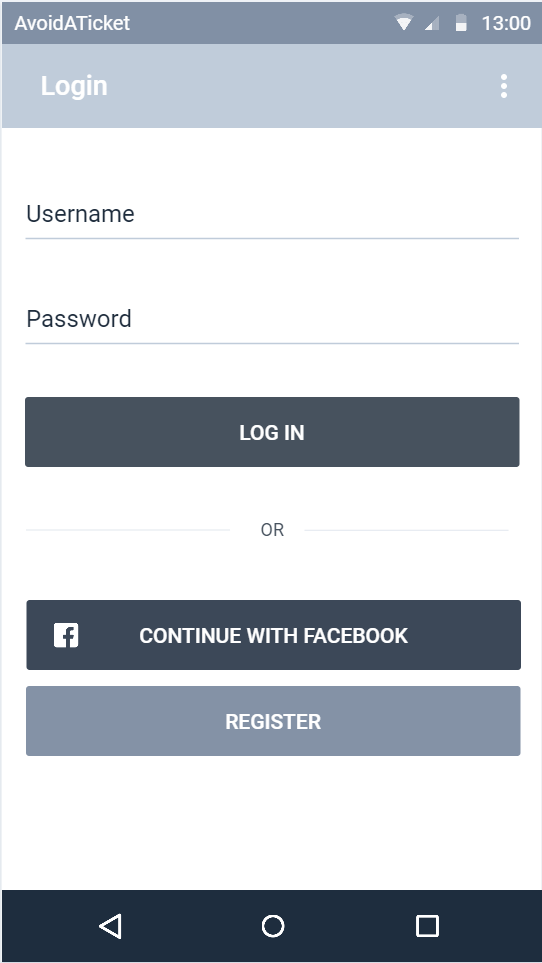
\includegraphics[scale=0.3]{img/mockup_login}
				\caption{Prisijungimo lango maketas}
				\label{img:prisijungimas}
			\end{figure}

\subsubsection{Profilio duomenų redagavimas}
	\textbf{Pagrindinis scenarijus:}\\
	Vartotojas pagrindiniame lange spaudžia mygtuką, ant kurio parašytas jo vardas ir pavardė, ir tada patenka į profilio 
	redagavimo langą. Ten iš el. pašto, slaptažodžio, vardo, pavardės laukų paspaudžia ant vardo lauko ir įveda naują vardą. 
	Tada paspaudžia mygtuką “Save” ir pakeisti duomenys išsaugomi duomenų bazėje. Vartotojas apie tai informuojamas informaciniu pranešimu. 
	Pakeitęs duomenis, vartotojas paspaudžia mygtuką “Back” ir grįžtą į pagrindinį langą.

	\textbf{Alternatyvūs scenarijai:}
	\begin{enumerate}[itemsep=-2mm]
		\item Jei įvestame slaptažodyje nėra skaičiaus ar didžiosios raidės, arba jis yra trumpesnis nei 5 simboliai, tada vartotojui programa pateikia informacinį pranešimą, kad slaptažodis netinkamas, jame privalo būti didžioji raidė ir skaičius ir kad jį turi sudaryti bent 5 simboliai.
		\item Jei vartotojo įvestas prisijungimo vardas duomenų bazėje jau egzistuoja, tada vartotojui programa pateikia informacinį pranešimą, kad prisijungimo vardas netinkamas, nes jau yra vartotojas su tokiu prisijungimo vardu.
		\item Jei vartotojo įvestame prisijungimo varde nėra 5 simbolių, programa pateikia informacinį pranešimą, kad prisijungimo vardas netinkamas, nes jame turi būti bent 5 simboliai.
		\item Jei vartotojo įvestas el. paštas neatitinka el. pašto formato, programa informuoja vartotoją, kad įvestas el. paštas netinkamas.
		\item Jei vartotojo įvestas prisijungimo vardas yra per ilgas, tada vartotojui programa pateikia informacinį pranešimą, kad prisijungimo vardas netinkamas, nes prisijungimo vardas negali būti ilgesnis nei 15 simbolių eilutė.
		\item Jei  vartotojo įvestas slaptažodis yra per ilgas, tada vartotojui programa pateikia informacinį pranešimą, kad slaptažodis netinkamas, nes slaptažodis negali būti ilgesnis nei 20 simbolių eilutė.
		\item Jei dėl trikdžių duomenų bazėje vartotojui pakeisti duomenų nepavyksta, tada vartotojui programa pateikia informacinį pranešimą, kad sistemoje įvyko klaida ir siūloma pabandyti prisiregistruoti vėliau.
	\end{enumerate} 
	\begin{figure}[H]
				\centering
				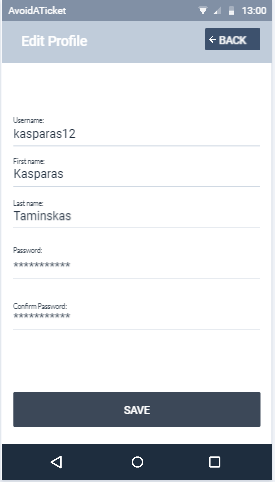
\includegraphics[scale=0.55]{img/mockup_profileedit}
				\caption{Profilio redagavimas}
				\label{img:profilio redagavimas}
			\end{figure}
\subsubsection{Komentaro apie žymeklį pridėjimas}
	\textbf{Pagrindinis scenarijus:}\\
    Vartotojas paspaudžia ant žymeklio, sistema jį nukelia į žymeklio informacijos langą. Vartotojas žymeklio informacijos lange 
	įrašo komentarą į tam skirtą laukelį, spaudžia “Siųsti”. Sistema įrašo komentarą apie žymeklį į duomenų bazę. Sistema 
	atvaizduoja komentarą komentarų sąrašo viršuje.

	\textbf{Alternatyvūs scenarijai:}
	\begin{enumerate}[itemsep=-2mm]
		\item Jei dėl trikdžių bandant pasiekti internetą, nepavyksta į duomenų bazę įrašyti vartotojo komentaro, tada vartotojui programa pateikia informacinį pranešimą, kad sistemoje įvyko klaida ir siūloma pabandyti vėliau.
	\end{enumerate} 
	\begin{figure}[H]
				\centering
				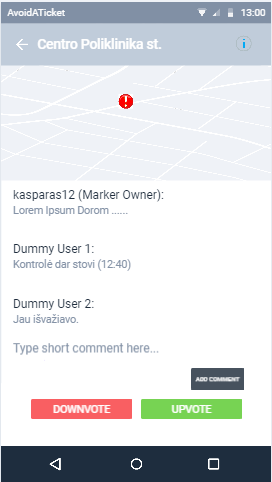
\includegraphics[scale=0.6]{img/mockup_markerInfoWindow}
				\caption{Žymeklio informacijos langas}
				\label{img:Žymeklio informacijos langas}
			\end{figure}

\subsubsection{Maršruto pridėjimas į sekamų sąrašą}
	\textbf{Pagrindinis scenarijus:}\\
	Vartotojas lange “Mano maršrutai” spaudžia “+” ir sistema atidaro bendrą miesto autobusų sąrašą, kuriame neįtraukti 
	vartotojo jau anksčiau pažymėti autobusai, kurių maršrutai įtraukti į sekamų sąrašą. Vartotojas paspaudžia ant jį 
	dominančio autobuso sąrašo elemento iš bendro miesto autobusų sąrašo, tada sistema įtraukia pasirinktą autobuso maršrutą 
	į vartotojo sekamų maršrutų sąrašą. Sistema parodo pranešimą pranešimų srityje “Autobuso {autobusas} maršrutas sėkmingai 
	įtrauktas į sekamų maršrutų sąrašą“. Sistema perkelia vartotoją i “Mano maršrutai” langą. Vartotojo pasirinktas autobuso 
	elementas atvaizduojamas “Mano maršrutai” lango sąrašo gale.

	\textbf{Alternatyvūs scenarijai:}
	\begin{enumerate}[itemsep=-2mm]
		\item Jei dėl trikdžių bandant pasiekti internetą, nepavyksta vartotojui parodyti bendrą autobusų sąrašą ar pridėti autobuso maršrutą į sekamų maršrutų sąrašą, tada vartotojui programa pateikia informacinį pranešimą, kad sistemoje įvyko klaida ir siūloma pabandyti vėliau.
	\end{enumerate} 
	\begin{figure}[H]
				\centering
				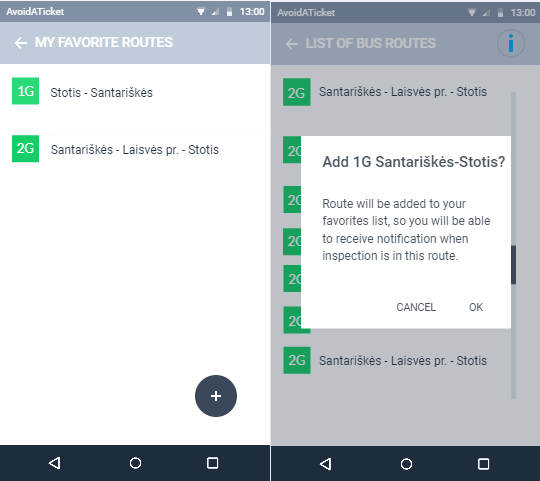
\includegraphics[scale=1.5]{img/mockup_AddRoute}
				\caption{Maršruto pridėjimo langas}
				\label{img:Maršruto pridėjimo langas}
			\end{figure}

\subsubsection{Atsijungimas}
	Šiame skyriuje aprašomas vartotojo atsijungimo nuo aplikacijos procesas, kuris yra schematizuotas robastiškumo diagramoje (žr. \ref{img:Atsijungimo robustiškumo diagrama} pav.).\\
	\textbf{Pagrindinis scenarijus:}\\
	Vartotojas pagrindiniame lange paspaudžia “Log Off”, sistema jį atjungia ir vartotojas yra nukeliamas į prisijungimo langą.
		\begin{figure}[H]
				\centering
				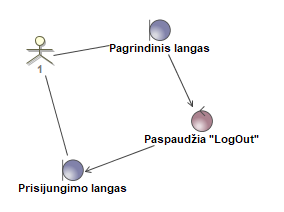
\includegraphics[scale=1]{img/Robustness_Atsijungimas}
				\caption{Atsijungimo robustiškumo diagrama}
				\label{img:Atsijungimo robustiškumo diagrama}
			\end{figure}

\subsubsection{Žemėlapio ir jame esančių žymeklių peržiūra}
	\textbf{Pagrindinis scenarijus:}\\
	Vartotojas pagrindiniame lange paspaudžia “Open Map” ir yra nukeliamas į žemėlapio langą, kuriame rodomi visi galiojantys žymekliai.

	\textbf{Alternatyvūs scenarijai:}
	\begin{enumerate}[itemsep=-2mm]
		\item Jei vartotojas neturi davęs sutikimo programėlei naudotis GPS, tada ji prašo prieigos prie GPS pateikdama informacijos langą.
		\begin{enumerate}[itemsep=-2mm]
			\item Jei vartotojas paspaudžia “Accept”, programėlei duodamas sutikimas naudotis telefono GPS ir vartotojas yra nukeliamas į žemėlapio langą, kuriame rodomi visi galiojantys žymekliai.
			\item Jei vartotojas paspaudžia “Decline”, programa pateikia informacinį pranešimą, kad negali parodyti žemėlapio, nes vartotojas nesuteikė prieigos prie GPS.
		\end{enumerate} 
		\item Jei programai nepavyksta rasti vartotojo buvimo vietos, tada vartotojui programa pateikia informacinį pranešimą, kad vartotojo buvimo vietos rasti nepavyko.
	\end{enumerate} 
	\begin{figure}[H]
				\centering
				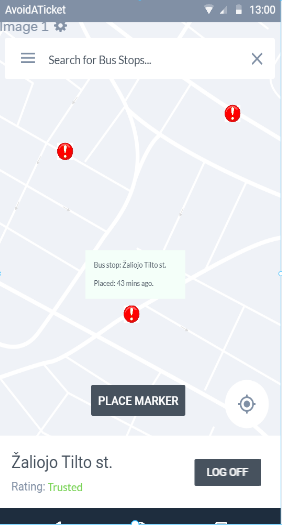
\includegraphics[scale=0.6]{img/mockup_Main_Window}
				\caption{Pagrindinis langas}
				\label{img:Pagrindinis langas}
			\end{figure}

\subsubsection{Žemėlapio redagavimas. Žymeklių pridėjimas}
	\textbf{Pagrindinis scenarijus:}\\
	Vartotojas pagrindiniame lange paspaudžia “Put Marker” ir yra nukeliamas į žymeklių pridėjimo langą, tada paspaudžia ant žemėlapio ir žymeklis yra padedamas toje vietoje, kur buvo paspausta.

	\textbf{Alternatyvūs scenarijai:}
	\begin{enumerate}[itemsep=-2mm]
		\item Jei vartotojas neturi davęs sutikimo programėlei naudotis GPS, tada ji prašo prieigos prie GPS pateikdama informacijos langą.
		\begin{enumerate}[itemsep=-2mm]
			\item Jei vartotojas paspaudžia “Accept”, programėlei duodamas sutikimas naudotis telefono GPS ir vartotojas yra nukeliamas į žymeklių pridėjimo langą, kuriame rodomi visi galiojantys žymekliai.
			\item Jei vartotojas paspaudžia “Decline”, programa pateikia informacinį pranešimą, kad negali parodyti žemėlapio, nes vartotojas nesuteikė prieigos prie GPS.
		\end{enumerate} 
		\item Jei programai nepavyksta rasti vartotojo buvimo vietos, tada vartotojui programa pateikia informacinį pranešimą, kad vartotojo buvimo vietos rasti nepavyko.
		\item Jei vartotojas bando padėti žymeklį vietoje, kuri yra nutolusi daugiau nei 1.5 km nuo vartotojo, tada vartotojui programa pateikia informacinį pranešimą, kad vartotojas negali dėti žymeklių vietose, nutolusiose nuo vartotojo per daugiau nei 1.5 km.
	\end{enumerate} 
	\begin{figure}[H]
				\centering
				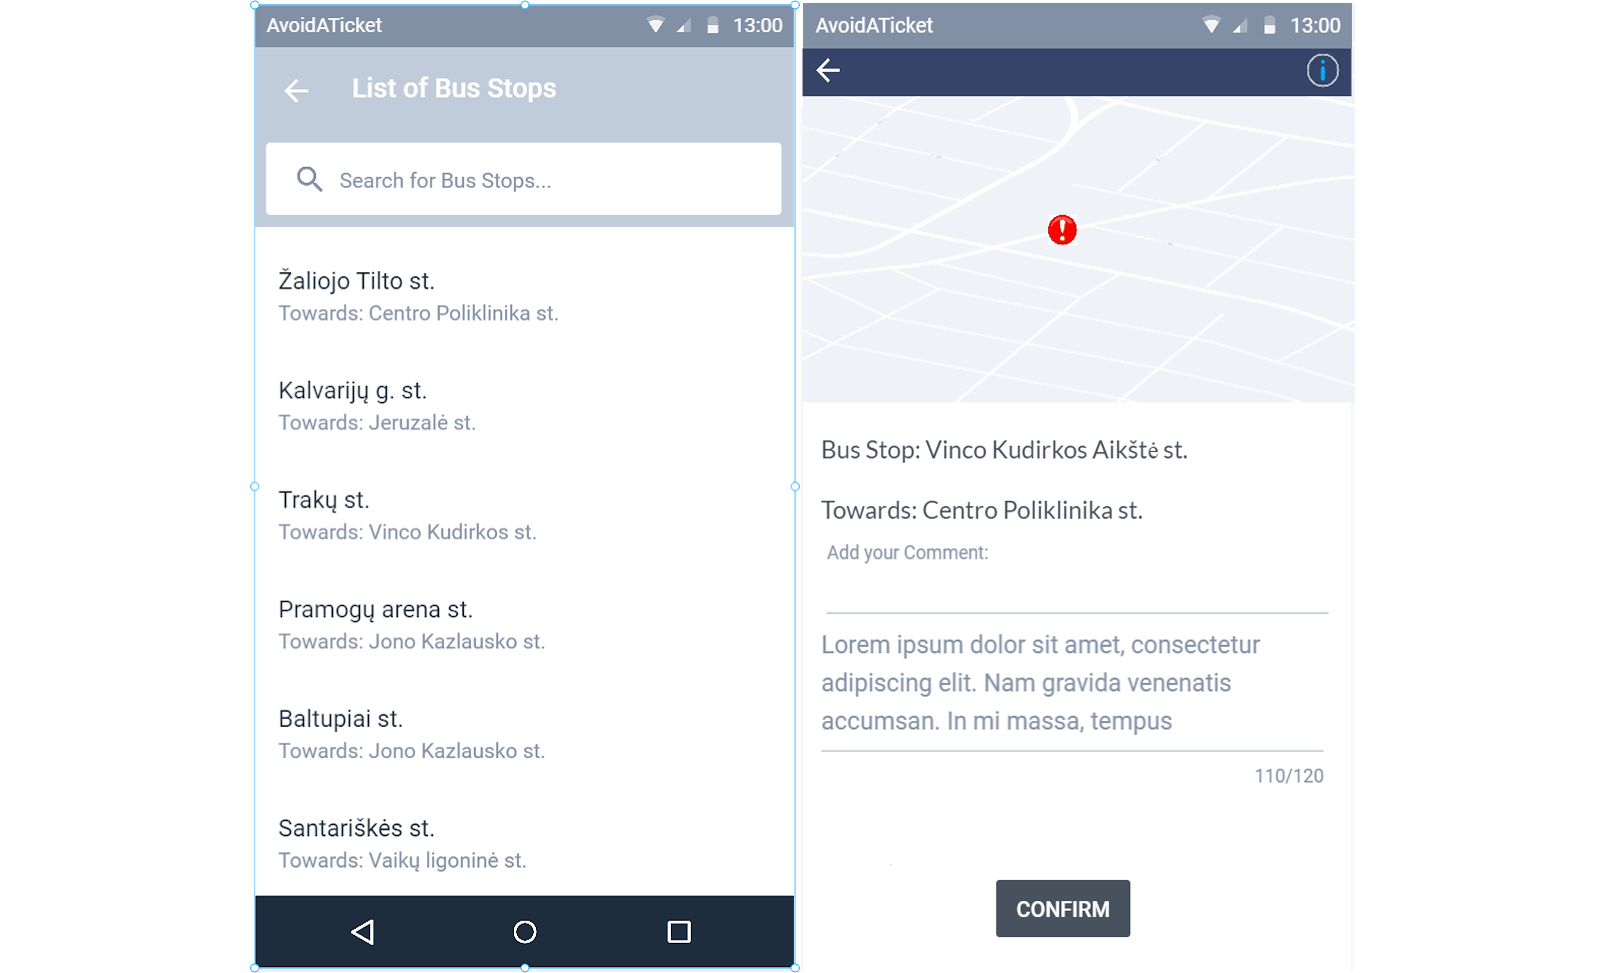
\includegraphics[scale=0.2]{img/mockup_AddMarker}
				\caption{Žymeklio pridėjimo langas}
				\label{img:Žymeklio pridėjimo langas}
			\end{figure}

\subsubsection{Žemėlapio redagavimas. Vartotojų balsavimas dėl žymeklio teisingumo}
	\textbf{Pagrindinis scenarijus:}\\
	Vartotojas pagrindiniame lange paspaudžia “Open Map” ir yra nukeliamas į žemėlapio langą, kuriame rodomi visi galiojantys žymekliai. 
	Vartotojas paspaudžia ant pasirinkto galiojančio žymeklio, kuris yra ne toliau nei 1,5km nuo jo dabartinės padėties ir yra nukeliamas 
	į žymeklio balsavimo langą. Jei kontrolė vartotojo pasirinkto žymeklio vietoje jau nebestovi, vartotojas paspaudžia mygtuką “Nestovi”, 
	sistema išsaugoja vartotojo balsą duomenų bazėje, žymintį, kad kontrolė pasitraukė iš pasirinkto žymeklio vietos. Jei kontrolė žymeklio 
	vietoje vis dar stovi, vartotojas paspaudžia mygtuką “Dar stovi” ir sistema išsaugo vartotojo balsą duomenų bazėje, patvirtinantį, kad 
	kontrolė dar yra pasirinkto žymeklio vietoje. Vartotojas, atidavęs savo balsą, yra perkeliamas į bendrą žemėlapio langą su visais 
	galiojančiais žymekliais. Žymeklio, gavusio 51% balsų, žyminčių, kad kontrolė žymeklio vietoje jau nebestovi, spalva yra pakeičiama į pilką.

	\textbf{Alternatyvūs scenarijai:}
	\begin{enumerate}[itemsep=-2mm]
		\item Jei vartotojas pasirenka žymeklį, esantį toliau nei 1,5km nuo jo esamos buvimo vietos, nustatytos pagal GPS, vartotojui nėra rodomas žymeklio balsavimo langas ir jam neleidžiama balsuoti.
		\item Jei programai nepavyksta rasti vartotojo buvimo vietos, tada vartotojui programa pateikia informacinį pranešimą, kad vartotojo buvimo vietos rasti nepavyko.
		\item Jei vartotojas bando balsuoti už tą patį žymeklį antrą kartą, sistema jam praneša, kad jis jau balsavo anksčiau ir neįskaito vartotojo balso.
	\end{enumerate} 
	\begin{figure}[H]
				\centering
				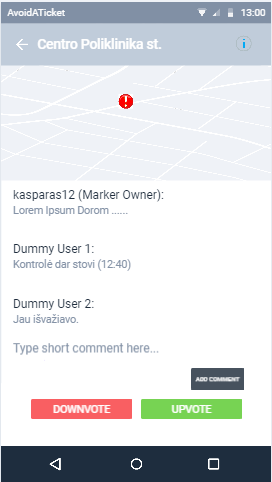
\includegraphics[scale=0.6]{img/mockup_markerInfoWindow}
				\caption{Žymeklio informacijos langas}
				\label{img:Žymeklio informacijos langas}
			\end{figure}

\subsubsection{Žemėlapio redagavimas. Žymeklių trynimas}
	\textbf{Pagrindinis scenarijus:}\\
	Administratorius pagrindiniame lange paspaudžia “Clear Markers”, tada programėlė ištrina visus žymeklius, esamus žemėlapyje.

	\textbf{Alternatyvūs scenarijai:}
	\begin{enumerate}[itemsep=-2mm]
		\item Jei dėl trikdžių nepavykstą ištrinti bent vieno žymeklių, ištrinti žymekliai yra grąžinami į savo vietas ir programėlė informuoja administratorių informaciniu pranešimu, kad dėl trikdžių duomenų bazėje nepavyko ištrinti žymeklių ir siūloma administratoriui pabandyti vėliau.
	\end{enumerate} 

\subsubsection{Susisiekimas su administracija}
	\textbf{Pagrindinis scenarijus:}\\
	Vartotojas pagrindiniame lange paspaudžia “FAQ | Ask a question” ir patenka į D.U.K. langą. D.U.K lange vartotojas 
	spaudžia “Ask a question” mygtuką ir patenka į klausimo uždavimo langą. Klausimo uždavimo lange vartotojas įveda 
	savo el. paštą ir klausimą bei spaudžia “Send us the question”. Klausimas nusiunčiamas sėkmingai, o programa informuoja 
	vartotoją, kad klausimą nusiųsti pavyko.

	\textbf{Alternatyvūs scenarijai:}
	\begin{enumerate}[itemsep=-2mm]
		\item Jei vartotojas el. pašto lauką palieka tuščią, programa informuoja vartotoją, kad klausimo nusiųsti nepavyko, nes vartotojas nepateikė savo el. pašto.
		\item Jei vartotojo įvestas el. paštas neatitinka el. pašto formato, programa informuoja vartotoją, kad įvestas el. paštas netinkamas.
		\item Jei vartotojas klausimo lauką palieka tuščią, programa informuoja vartotoją, kad klausimo nusiųsti nepavyko, nes vartotojas klausimo lauką paliko tuščią.
	\end{enumerate} 
	\begin{figure}[H]
				\centering
				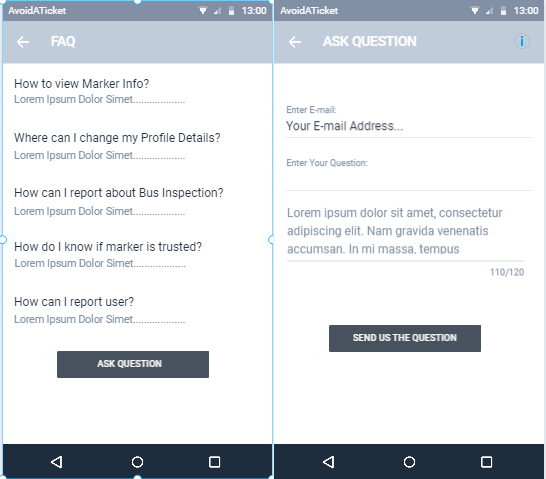
\includegraphics[scale=1.4]{img/mockup_admincomunication}
				\caption{Susisiekimas su administracija}
				\label{img:Susisiekimas su administracija}
			\end{figure}
\subsection{Reikalavimų - užduočių atsekamumo matrica}
	\begin{figure}[H]
				\centering
				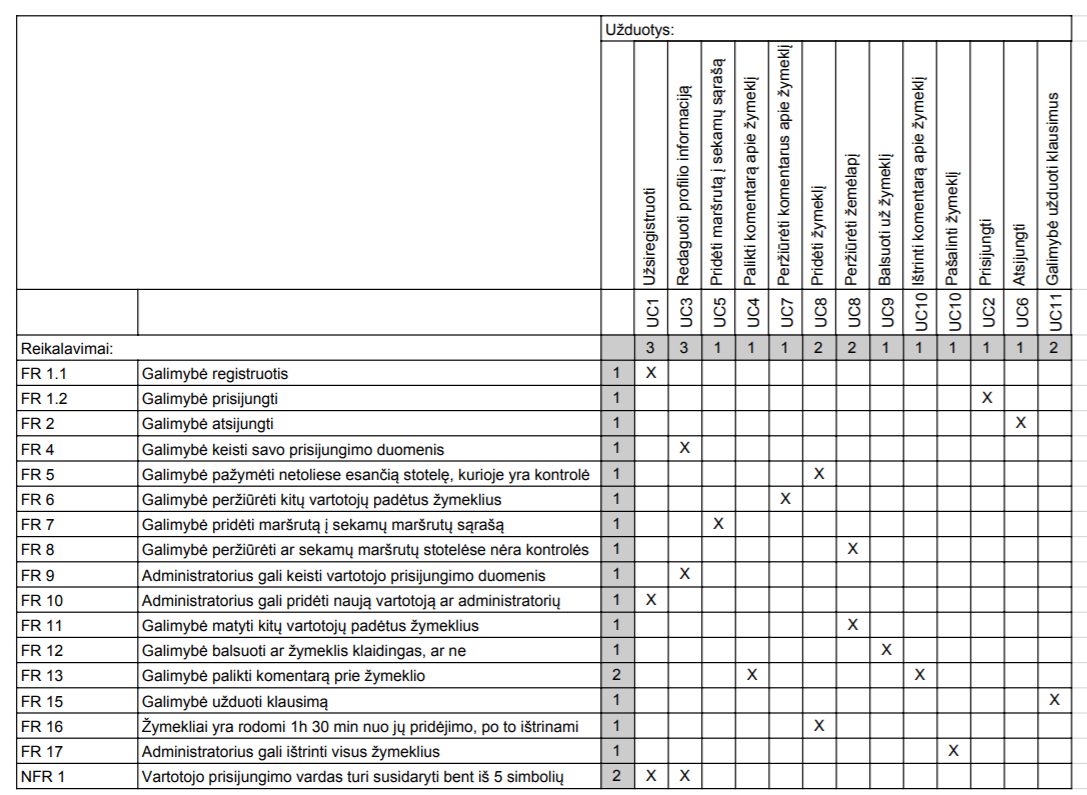
\includegraphics[scale=0.4]{img/uzduociu_matrica}
				\caption{Užduočių atsekamumo matrica}
				\label{img:matrix}
			\end{figure}
			
\section{Poreikiai}
\subsection{Išoriniai komponentai}

\begin{figure}[H]
	\centering
	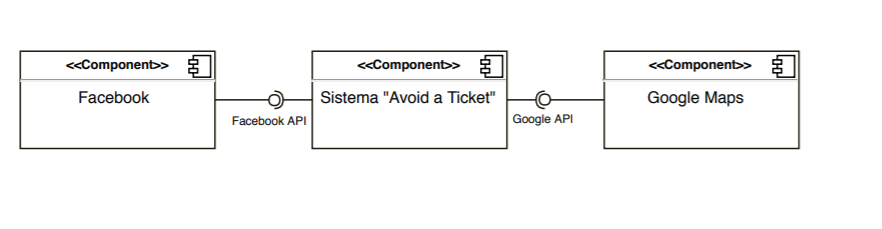
\includegraphics[scale=0.7]{img/Isoriniai_komponentai}
	\caption{Išoriniai komponentai}
	\label{img:matrix}
\end{figure}

Sistema jungiasi prie Facebook, kai norima prisijungti prie programėlės per Facebook paskyrą.
Sistema jungiasi prie Google Maps, kad būtų matomas žemėlapis, kuriame žymimos kontrolės vietos, rodomi maršrutai ir stotelės (žr 17 pav.)


\subsection{Vidiniai komponentai}

\begin{figure}[H]
	\centering
	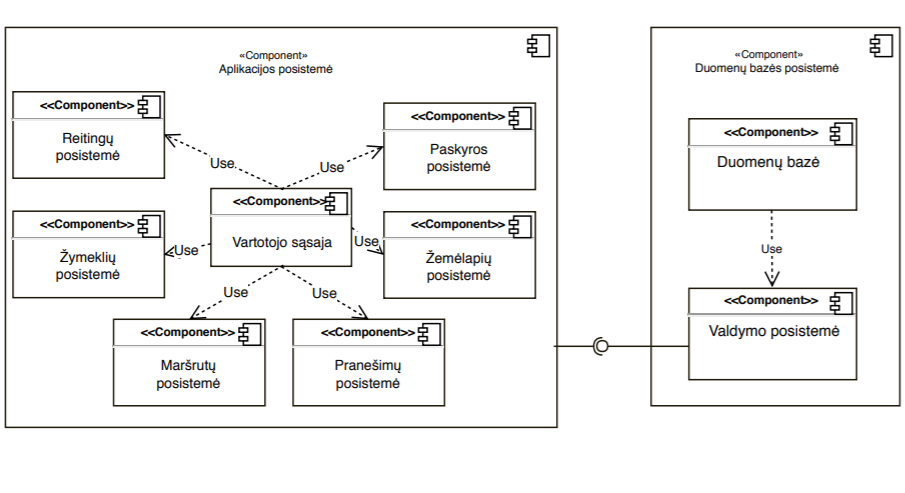
\includegraphics[scale=0.7]{img/Vidiniai_komponentai}
	\caption{Vidiniai komponentai}
	\label{img:matrix}
\end{figure}

Avoid a Ticket sistemą sudaro dvi posistemės - aplikacijos ir duomenų bazės posistemė. Duomenų bazės posistemėje yra duomenų bazė, kur saugomi sistemos duomenys, ir valdymo posistemė, kuri atlieka duomenų bazių ir kitas užklausas bei jungiasi su aplikacijos posisteme.Aplikacijos posistemėje yra vartotojo sąsaja, kuri pasitelkdama likusias posistemes (paskyros, žemėlapių, pranešimų, maršrutų, žymeklių ir reitingų) ir jų metodus parūpina informaciją vartotojui bei pateikia ją grafiniu būdu (žr 18 pav.).

\subsection{Komponentų išsidėstymas tinkle, jų saugumas}

\begin{figure}[H]
	\centering
	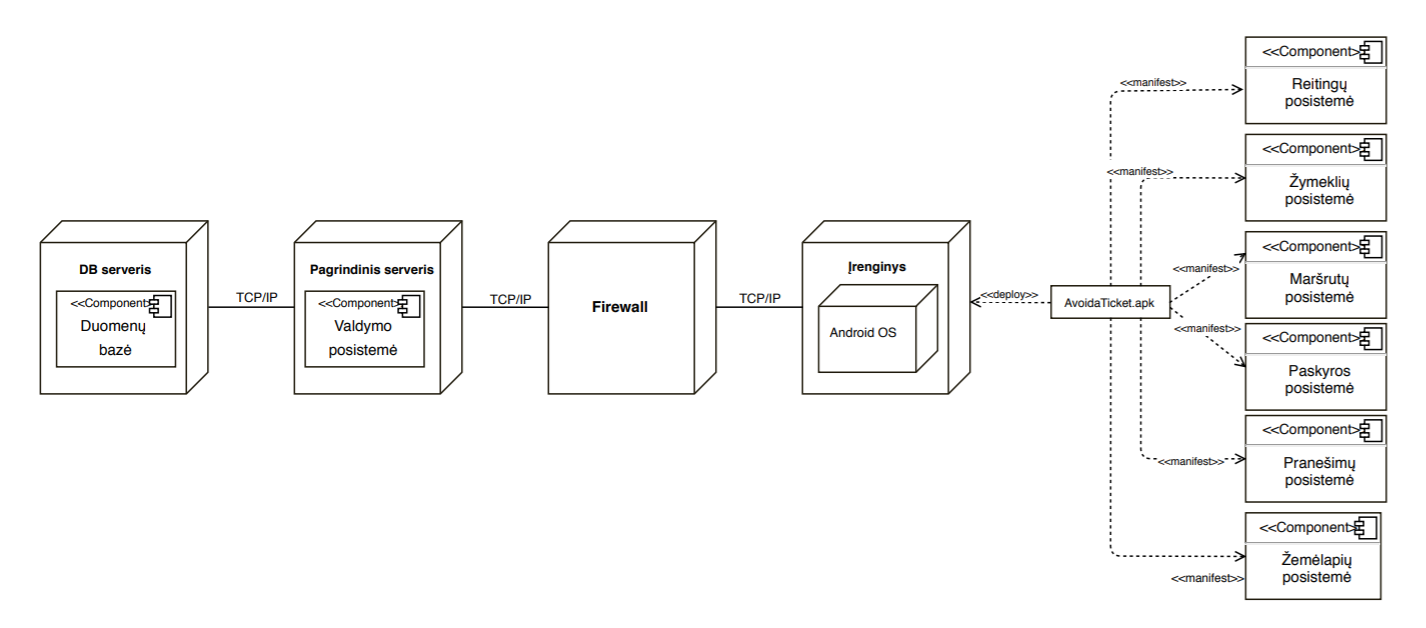
\includegraphics[scale=0.4]{img/Komponentu_issidestymas}
	\caption{Komponentų išsidėstymas}
	\label{img:matrix}
\end{figure}

Avoid a Ticket sistemoje yra du serveriai, viename jų yra duomenų bazė su duomenimis, kitame – valdymo posistemė, kuri valdo duomenų srautą sistemoje. Taip pat yra
įrenginys su įrašyta android operacine sistema bei Avoid a Ticket aplikacija, kurioje veikia anksčiau minėtos posistemės. Įrenginio naudotojas gali būti administratorius arba klientas. Įrenginiai su pagrindiniu serveriu bei duomenų bazės ir pagrindinis serveriai tarpusavyje siejasi TCP/IP ryšiu, kurio srautą prižiūri „Firewall“ mazgas saugodamas nuo nuotolinių atakų – bandymo išgauti duomenis, kenkėjiškų programų palikimo ar kitos potencialios žalos sistemai (žr 19 pav.).

\subsection{Diegimas ir palaikymas}

Aplikacija talpinama Google „Play Store“ sistemoje, iš kurios kiekvienas asmuo su Android operacinę sistemą palaikančiu įrenginiu gali ją atsisiųsti. Aplikacijos atnaujinimai vyksta taip pat per Google „Play Store“. Vartotojai, pirmą kartą diegiantys programėlę, siunčiasi naujausią tuo metu prieinamą versiją, o atnaujinimo atveju turi galimybę atsisiųsti naujesnę
versiją ir ja pakeisti senesnę.


\section{Rastų klaidų sąrašas}
	\begin{enumerate}[itemsep=-2mm]
		\item Struktūriniame esybių modelyje nebuvo Maršruto esybės.
		\item Struktūriniame esybių modelyje Filtro esybė buvo agregacijos ryšiu sujungta su žymekliu.
		\item Struktūriniame dalykinės srities modelyje buvo naudojamos ne tik agregacijos ir generalizacijos.
		\item Netikslus funkcinis reikalavimas, nusakantis, kiek laiko po žymeklio pridėjimo jis yra matomas vartotojams.
		\item Užduočių aprašymuose naudojama ne tik tiesioginė nuosaka.
		\item Struktūriniame esybių modelyje nebuvo atskirų Paskiros ir “Facebook” paskyros esybių.
		\item Nebuvo sunumeruoti paveikslėliai.
		\item Nebuvo funkcinio reikalavimo vartotojo galimybei pasirinkti maršrutą ir tikrinti stoteles pagal jį.
		\item Nebuvo funkcinio reikalavimo vartotojo galimybei filtruoti matomus žymeklius pagal pasirinktą maršrutą.
		\item Netiksliai aprašytas poreikis, kokiu atstumu nuo vartotojo buvimo vietos, jis gali padėti žymeklį.
	\end{enumerate}
\sectionnonum{Išvada}
Šiame etape sukurta įvadinė verslo taisyklių logika leidžia toliau sėkmingai detalizuoti sistemos komponentus pereinant į žemesnius abstrakcijos lygius - sistemą galima skaidyti į atskirus verslo esybių modulius ir kiekvieną jų nagrinėti atskirai. Kadangi ICONIX proceso esmė - klaidinga kiekvienos iteracijos įeiga, todėl nereikia baimintis likusių neapibrėžtumų ir abstraktumo - visa tai bus detalizuota kitų laboratorinių darbų metu.

\sectionnonum{Literatūros sąrašas}
\begin{enumerate}[label={[\arabic*]};itemsep=-2mm]
	\item Doc. dr. K. Petrausko Programų Sistemų Inžinerijos kurso konspektai
	\item Doug Rosenberg and Matt Stephens - „Use Case Driven Object Modeling with UML Theory and Practice“
	\item UML dokumentacija \url{https://www.tutorialspoint.com/uml/uml_2_overview.htm}
	\item OMG UML v.2.5 Dokumentacija diagramoms, žymėjimui
\end{enumerate}

\end{document}
